% Options for packages loaded elsewhere
\PassOptionsToPackage{unicode}{hyperref}
\PassOptionsToPackage{hyphens}{url}
%
\documentclass[
]{article}
\usepackage{amsmath,amssymb}
\usepackage{iftex}
\usepackage{tikz}
\ifPDFTeX
  \usepackage[T1]{fontenc}
  \usepackage[utf8]{inputenc}
  \usepackage{textcomp} % provide euro and other symbols
\else % if luatex or xetex
  \usepackage{unicode-math} % this also loads fontspec
  \defaultfontfeatures{Scale=MatchLowercase}
  \defaultfontfeatures[\rmfamily]{Ligatures=TeX,Scale=1}
\fi
\usepackage{lmodern}
\ifPDFTeX\else
  % xetex/luatex font selection
\fi
% Use upquote if available, for straight quotes in verbatim environments
\IfFileExists{upquote.sty}{\usepackage{upquote}}{}
\IfFileExists{microtype.sty}{% use microtype if available
  \usepackage[]{microtype}
  \UseMicrotypeSet[protrusion]{basicmath} % disable protrusion for tt fonts
}{}
\makeatletter
\@ifundefined{KOMAClassName}{% if non-KOMA class
  \IfFileExists{parskip.sty}{%
    \usepackage{parskip}
  }{% else
    \setlength{\parindent}{0pt}
    \setlength{\parskip}{6pt plus 2pt minus 1pt}}
}{% if KOMA class
  \KOMAoptions{parskip=half}}
\makeatother
\usepackage{xcolor}
\usepackage{graphicx}
\makeatletter
\def\maxwidth{\ifdim\Gin@nat@width>\linewidth\linewidth\else\Gin@nat@width\fi}
\def\maxheight{\ifdim\Gin@nat@height>\textheight\textheight\else\Gin@nat@height\fi}
\makeatother
% Scale images if necessary, so that they will not overflow the page
% margins by default, and it is still possible to overwrite the defaults
% using explicit options in \includegraphics[width, height, ...]{}
\setkeys{Gin}{width=\maxwidth,height=\maxheight,keepaspectratio}
% Set default figure placement to htbp
\makeatletter
\def\fps@figure{htbp}
\makeatother
\setlength{\emergencystretch}{3em} % prevent overfull lines
\providecommand{\tightlist}{%
  \setlength{\itemsep}{0pt}\setlength{\parskip}{0pt}}
\setcounter{secnumdepth}{-\maxdimen} % remove section numbering
\ifLuaTeX
  \usepackage{selnolig}  % disable illegal ligatures
\fi
\IfFileExists{bookmark.sty}{\usepackage{bookmark}}{\usepackage{hyperref}}
\IfFileExists{xurl.sty}{\usepackage{xurl}}{} % add URL line breaks if available
\urlstyle{same}
\hypersetup{
  hidelinks,
  pdfcreator={LaTeX via pandoc}}

\author{}
\date{}

\begin{document}

\section{Reading 2}\label{reading-2}

\subsection{Problem 1) Provide a summary of your understanding of
recurrence ( what recurrence is, how to solve recurrences and give an
example).}\label{problem-1-provide-a-summary-of-your-understanding-of-recurrence--what-recurrence-is-how-to-solve-recurrences-and-give-an-example}

Recurrence implies repetition. In algorithms, recurrence is the process
of repeatedly applying a function to break down a problem into smaller
sub-problems till a \emph{base case} is reached. A base case is the
point where the recurrence terminates ; i.e.; the recurrence function
does not call itself anymore. It \emph{usually} is represented by a case
that is elementary in nature and cannot be further broken down into
sub-cases.

A recurrence equation is a mathematical representation of a recurrence
condition. This equation defines a function which is defined in terms of
their previous values. Recurrence equations are widely used during
algorithmic analysis of recurrence based algorithms, specially divide
and conquer algorithms.

It is necessary to determine whether the problem can be broken down into
smaller instances of the same problem in order to formulate a recursive
problem.\\
Conquer the subproblems by solving them recursively. Solve the
subproblem on reaching the base case, then combine the subproblem
solutions to get the answer to the original problem.

An example of a recurrence equation is \(T(n) = 2T(n/2)\). This equation
is balanced, as in it divides the input problem into an equal number of
subproblems. We can visualize this through a recurrence tree which are
the same in value.

As we can see, each node is divided into 2 child nodes

However, recurrence equations can also be
\textquotesingle unbalanced\textquotesingle{} or produce subproblems
that are inequal. An example of such an equation is S

\subsection{Problem 2) Give an example of a recurrence equation from a
problem that you have studied (e.g Convex Hull, Quicksort, Matrix
Multiplication etc) and show how this is solved
using:}\label{problem-2-give-an-example-of-a-recurrence-equation-from-a-problem-that-you-have-studied-eg-convex-hull-quicksort-matrix-multiplication-etc-and-show-how-this-is-solved-using}

\subsubsection{1. Recursion tree}\label{1-recursion-tree}

Let\textquotesingle s consider merge sort, whose recurrence equation we
are familiar with :

\(T(n) = 2T(n/2) + O(n)\)

This means the tree has a branching factor of 2 (splits into 2 parts on
each level) and splits into children of n/2 the original parent. We can
draw the tree as following:

\begin{figure}
  \centering
  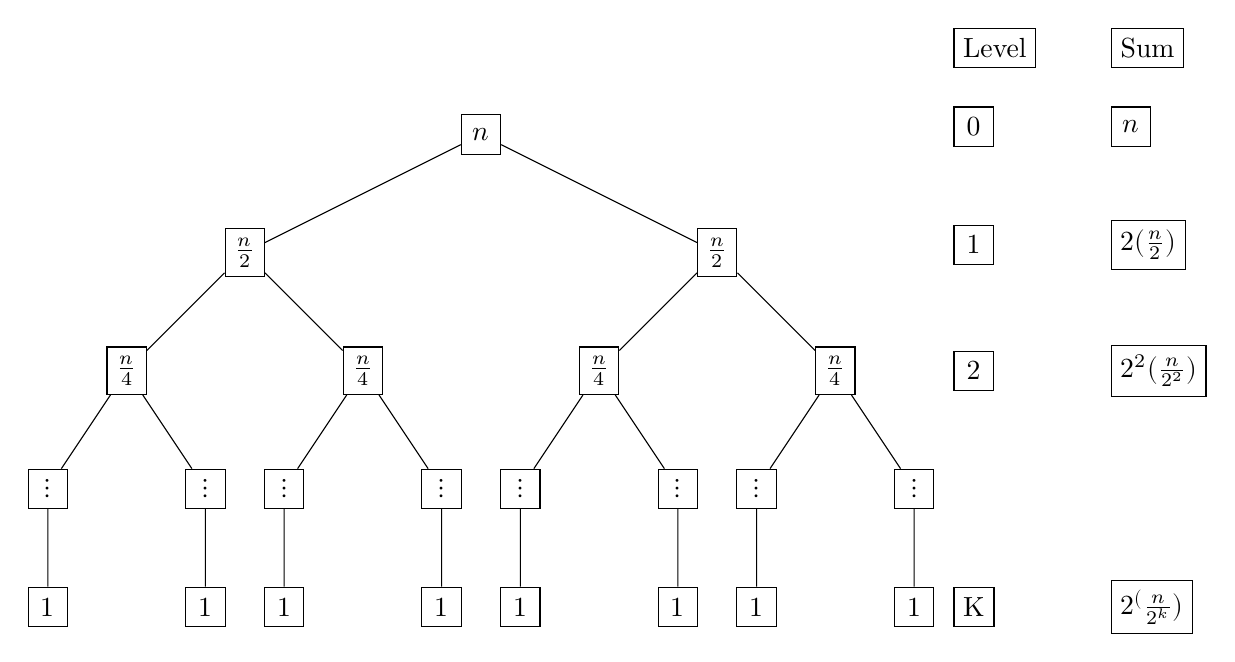
\begin{tikzpicture}[
    level/.style={sibling distance=60mm/#1},
    every node/.style={draw, rectangle, minimum size=5mm},
  ]
  \node {$n$} 
    child {
      node {$\frac{n}{2}$}
      child {
        node {$\frac{n}{4}$}
        child {
          node {$\vdots$}
          child{
          node{$1$}
          }
        }
        child {
          node {$\vdots$}
          child{
          node{$1$}
          }
        }
      }
      child {
        node {$\frac{n}{4}$}
        child {
          node {$\vdots$}
          child{
          node{$1$}
          }
        }
        child {
          node {$\vdots$}
          child{
          node{$1$}
          }
        }
      }
    }
    child {
      node {$\frac{n}{2}$}
      child {
        node {$\frac{n}{4}$}
        child {
          node {$\vdots$}
          child{
          node{$1$}
          }
        }
        child {
          node {$\vdots$}
          child{
          node{$1$}
          }
        }
      }
      child {
        node {$\frac{n}{4}$}
        child {
          node {$\vdots$}
          child{
          node{$1$}
          }
        }
        child {
          node {$\vdots$}
          child{
          node{$1$}
          }
        }
      }
    };
    \node[anchor=west] at (6,1.1) {Level};
    \node[anchor=west] at (8,1.1) {Sum};
    \node[anchor=west] at (6,0.1) { 0};
    \node[anchor=west] at (8,0.1) {$n$};
    \node[anchor=west] at (6,-1.4) { 1};
    \node[anchor=west] at (8,-1.4) {$2(\frac{n}{2})$};
    \node[anchor=west] at (6,-3) {2};
    \node[anchor=west] at (8,-3) {$2^2(\frac{n}{2^2})$};
    \node[anchor=west] at (6,-6) {K};
    \node[anchor=west] at (8,-6) {$2^(\frac{n}{2^k})$};
  \end{tikzpicture}
  \end{figure}
  

Now, we can see that at level k, we reach our base case.

Hence :

\[\frac{n}{2^k} = 1 \\ 

\Rarr n = 2^k \\

k = log_2n\\\]

\(T_c = I_c+L_c\) Where \(I_c\) = branch complexity and \(L_c\) = leaf
node complexity.

\[I_c = \sum_{i=0}^{k = log(n)-1} 2^i(\frac{n}{2^i}) = n(logn-1) = nlogn - n \\

L_c = 2^k(\frac{n}{2^k}) = n\\

T_c = nlogn - n +n = nlogn\\\\

T(n) = O(nlogn)\]

\subsubsection{2. Master Theorem}\label{2-master-theorem}

Let us consider merge sort for this problem.

From Page 74 of CLRS, we know the recurrence equation for merge sort is
:

\[T(n) = 2T(\frac{n}{2})+O(n)\]

We have a generalized recurrence equation of the form :

\[T(n) = aT(n/b) + f(n)\]

To apply master theorem we must find out the variables \(a\) and \(b\)
as well as \(f(n)\).

Comparing our recurrence equation for merge sort we can identify
\(a=2\), \(b =2\), and \(f(n) = n\).

Now applying master theorem, we have \(log_ba = log_2(2) = 1\)

Since \(n^{log_ba}= n^{log_2(2)} = n\), which is also equal to \(f(n)\).

Hence case 2 of the master theorem applies and \(T(n) = \Theta(nlogn)\).

\subsection{Problem 3) Provide a quick review of Selection, Insertion,
Merge sort and quick sort and provide a summary of the O, Omega and
Theta asymptotic running times. These could come from your reading , you
do not need to compute
them.}\label{problem-3-provide-a-quick-review-of-selection-insertion-merge-sort-and-quick-sort-and-provide-a-summary-of-the-o-omega-and-theta-asymptotic-running-times-these-could-come-from-your-reading--you-do-not-need-to-compute-them}

\end{document}
